

\SourceLeaf{222}%
\Needspace{7\baselineskip}
\begin{center}
\textsc{Gauss} an \textsc{Schumacher}. Göttingen, 12. Juli 1831.
\end{center}

\mbox{.\ .\ .\ .\ .\ .\ .} Was die Parallellinien betrifft, so würde ich Ihnen mein Urtheil sehr gern schon auf Ihren ersten Brief geschrieben haben, wenn ich nicht hätte voraussetzen müssen, dass Ihnen mit demselben ohne vollständige Entwickelungen wenig gedient sein würde. Zu solchen vollständigen Entwickelungen, wenn sie wahrhaft überzeugend sein sollen, würden aber vielleicht Bogenlange 
Auseinandersetzungen in Erwiederung auf das, was Sie in wenigen Zeilen im Grunde nur angedeutet haben, nöthig sein, zu welchen Auseinandersetzungen mir aber gegenwärtig die erforderliche Geistesheiterkeit fehlt. Um Ihnen jedoch meinen guten Willen zu bethätigen, will ich folgendes hersetzen.

Die eigentliche Pointe richten Sie sogleich auf jedes Dreieck; allein Sie würden im Grunde Ihr nemliches Räsonnement anwenden, wenn Sie das Geschäft zuerst auf den einfachsten Fall anwendeten und den Satz aufstellten:

1) In jedem Dreieck, dessen eine Seite endlich, die zweite und folglich auch die dritte hingegen unendlich ist, ist die Summe der beiden Winkel an jener $=180^0$.

\begin{center}
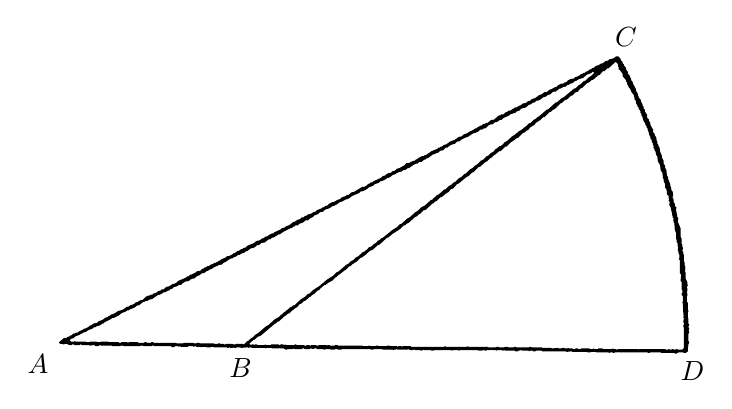
\begin{tikzpicture}[x=0.00720000cm,y=-0.00720000cm]
\fill[even odd rule] (1173,358) -- (1170,355) -- (1170,351) -- (1168,348) -- (1168,344) -- (1166,340) -- (1166,338) -- (1167,337) -- (1166,329) -- (1164,327) -- (1163,321) -- (1162,320) -- (1162,317) -- (1161,316) -- (1161,314) -- (1158,307) -- (1158,304) -- (1156,301) -- (1155,291) -- (1153,288) -- (1153,284) -- (1150,280) -- (1150,275) -- (1147,269) -- (1147,266) -- (1144,259) -- (1143,252) -- (1141,249) -- (1141,247) -- (1139,245) -- (1139,241) -- (1138,240) -- (1137,233) -- (1135,231) -- (1134,227) -- (1131,224) -- (1132,221) -- (1127,212) -- (1127,209) -- (1124,204) -- (1124,202) -- (1121,199) -- (1121,194) -- (1117,188) -- (1117,185) -- (1115,183) -- (1115,180) -- (1113,178) -- (1113,176) -- (1110,170) -- (1110,168) -- (1106,163) -- (1106,161) -- (1105,160) -- (1104,155) -- (1102,153) -- (1101,148) -- (1096,139) -- (1096,137) -- (1093,133) -- (1093,130) -- (1091,128) -- (1091,126) -- (1087,121) -- (1087,118) -- (1085,116) -- (1083,110) -- (1080,107) -- (1080,105) -- (1078,103) -- (1078,101) -- (1075,98) -- (1074,95) -- (1070,91) -- (1066,91) -- (1064,93) -- (1060,95) -- (1055,96) -- (1051,99) -- (1048,99) -- (1043,103) -- (1039,104) -- (1035,107) -- (1033,107) -- (1029,109) -- (1027,111) -- (1025,111) -- (1022,114) -- (1020,114) -- (1016,117) -- (1013,118) -- (1011,120) -- (1009,120) -- (1007,122) -- (1005,122) -- (1001,125) -- (997,127) -- (995,127) -- (992,130) -- (986,131) -- (982,133) -- (978,137) -- (975,137) -- (973,139) -- (970,139) -- (964,142) -- (961,145) -- (959,145) -- (952,149) -- (950,149) -- (944,154) -- (940,154) -- (935,158) -- (931,159) -- (923,165) -- (921,165) -- (917,167) -- (915,169) -- (911,170) -- (908,173) -- (902,174) -- (897,178) -- (895,178) -- (891,181) -- (888,181) -- (886,183) -- (884,183) -- (881,186) -- (876,187) -- (874,189) -- (871,190) -- (868,193) -- (864,193) -- (862,195) -- (860,195) -- (850,203) -- (846,203) -- (840,208) -- (838,208) -- (835,210) -- (832,210) -- (829,213) -- (827,213) -- (825,215) -- (823,215) -- (820,218) -- (818,218) -- (814,221) -- (807,224) -- (805,226) -- (797,229) -- (794,232) -- (789,233) -- (782,238) -- (774,241) -- (767,246) -- (763,247) -- (759,250) -- (757,250) -- (755,252) -- (753,252) -- (751,254) -- (741,258) -- (731,265) -- (729,265) -- (727,267) -- (724,267) -- (718,270) -- (716,272) -- (713,273) -- (711,275) -- (709,275) -- (701,279) -- (697,279) -- (693,283) -- (684,288) -- (680,289) -- (676,293) -- (673,293) -- (668,297) -- (665,297) -- (661,299) -- (659,301) -- (655,302) -- (652,305) -- (639,311) -- (637,313) -- (634,313) -- (632,315) -- (629,316) -- (626,319) -- (622,321) -- (619,321) -- (604,330) -- (599,331) -- (595,335) -- (592,335) -- (590,337) -- (582,340) -- (579,343) -- (577,343) -- (568,348) -- (566,348) -- (560,351) -- (557,354) -- (553,355) -- (551,357) -- (549,357) -- (547,359) -- (539,362) -- (536,365) -- (533,365) -- (531,367) -- (527,369) -- (524,369) -- (520,372) -- (518,372) -- (515,375) -- (512,375) -- (509,378) -- (505,379) -- (499,383) -- (497,383) -- (491,388) -- (487,390) -- (485,390) -- (483,392) -- (479,394) -- (477,394) -- (475,396) -- (464,401) -- (462,403) -- (460,403) -- (454,406) -- (452,408) -- (448,409) -- (444,412) -- (442,412) -- (440,414) -- (436,416) -- (434,416) -- (430,418) -- (428,420) -- (416,425) -- (413,428) -- (409,429) -- (407,431) -- (405,431) -- (401,434) -- (399,434) -- (394,438) -- (392,438) -- (390,440) -- (384,443) -- (381,443) -- (377,446) -- (370,449) -- (368,451) -- (366,451) -- (364,453) -- (360,455) -- (358,455) -- (356,457) -- (352,458) -- (348,461) -- (345,461) -- (343,463) -- (341,463) -- (339,465) -- (336,466) -- (333,469) -- (327,470) -- (325,472) -- (317,476) -- (315,476) -- (312,479) -- (310,479) -- (308,481) -- (294,487) -- (291,490) -- (287,492) -- (285,492) -- (277,497) -- (274,497) -- (268,502) -- (265,502) -- (263,504) -- (259,505) -- (255,508) -- (251,509) -- (249,511) -- (246,511) -- (243,513) -- (241,513) -- (237,515) -- (232,520) -- (225,522) -- (223,524) -- (219,525) -- (217,527) -- (213,529) -- (211,529) -- (207,532) -- (203,533) -- (196,538) -- (188,540) -- (184,543) -- (178,546) -- (176,546) -- (174,548) -- (171,549) -- (169,551) -- (167,551) -- (160,556) -- (154,558) -- (151,561) -- (145,562) -- (141,565) -- (138,566) -- (136,568) -- (130,571) -- (128,571) -- (126,573) -- (119,576) -- (117,578) -- (114,578) -- (111,580) -- (109,580) -- (106,583) -- (104,583) -- (102,585) -- (100,585) -- (96,588) -- (92,588) -- (89,591) -- (88,591) -- (84,595) -- (84,596) -- (86,598) -- (90,598) -- (91,599) -- (93,599) -- (94,598) -- (98,598) -- (102,600) -- (106,600) -- (107,599) -- (110,599) -- (111,600) -- (120,600) -- (121,599) -- (123,599) -- (124,600) -- (137,600) -- (138,601) -- (146,600) -- (149,602) -- (153,602) -- (156,600) -- (158,601) -- (177,601) -- (178,602) -- (192,602) -- (193,601) -- (197,601) -- (198,602) -- (227,602) -- (228,601) -- (232,601) -- (233,602) -- (247,602) -- (248,601) -- (251,601) -- (252,602) -- (257,602) -- (259,601) -- (260,602) -- (281,602) -- (284,604) -- (288,603) -- (289,602) -- (294,602) -- (295,603) -- (297,602) -- (299,603) -- (311,603) -- (312,602) -- (320,602) -- (322,603) -- (323,602) -- (325,602) -- (326,603) -- (334,603) -- (335,604) -- (337,603) -- (343,603) -- (344,604) -- (351,604) -- (352,603) -- (356,603) -- (357,604) -- (380,604) -- (381,605) -- (383,605) -- (384,604) -- (386,605) -- (390,605) -- (391,604) -- (393,605) -- (396,605) -- (397,604) -- (404,604) -- (405,605) -- (417,604) -- (419,605) -- (420,604) -- (423,604) -- (424,605) -- (447,605) -- (448,606) -- (450,605) -- (459,605) -- (460,606) -- (471,606) -- (473,605) -- (474,606) -- (480,606) -- (484,608) -- (486,608) -- (487,607) -- (496,607) -- (497,606) -- (499,607) -- (512,607) -- (513,606) -- (516,606) -- (517,607) -- (526,607) -- (527,606) -- (533,607) -- (534,606) -- (538,606) -- (539,607) -- (550,607) -- (551,608) -- (553,608) -- (554,607) -- (562,607) -- (563,608) -- (570,608) -- (571,607) -- (575,607) -- (576,608) -- (582,608) -- (583,607) -- (633,607) -- (634,608) -- (638,608) -- (639,607) -- (654,607) -- (655,608) -- (672,608) -- (673,609) -- (675,608) -- (678,608) -- (679,607) -- (681,608) -- (698,608) -- (700,607) -- (703,609) -- (708,609) -- (709,608) -- (711,608) -- (712,609) -- (721,609) -- (722,610) -- (724,610) -- (726,608) -- (728,609) -- (740,609) -- (741,610) -- (744,610) -- (745,609) -- (776,609) -- (777,610) -- (779,609) -- (788,609) -- (789,610) -- (791,609) -- (823,609) -- (824,610) -- (830,610) -- (831,609) -- (834,609) -- (835,610) -- (837,610) -- (838,609) -- (844,609) -- (846,608) -- (847,609) -- (854,609) -- (855,610) -- (857,609) -- (865,609) -- (866,610) -- (870,609) -- (871,610) -- (888,610) -- (889,611) -- (893,611) -- (894,610) -- (900,609) -- (901,610) -- (912,610) -- (913,611) -- (915,610) -- (919,610) -- (920,611) -- (924,611) -- (925,610) -- (935,610) -- (936,611) -- (978,611) -- (979,612) -- (988,611) -- (989,612) -- (1015,612) -- (1016,613) -- (1021,613) -- (1022,612) -- (1031,612) -- (1032,613) -- (1053,613) -- (1054,614) -- (1056,613) -- (1060,613) -- (1061,614) -- (1063,614) -- (1064,613) -- (1069,613) -- (1070,612) -- (1072,613) -- (1122,613) -- (1123,614) -- (1125,614) -- (1126,613) -- (1145,613) -- (1146,614) -- (1169,614) -- (1170,615) -- (1173,615) -- (1176,613) -- (1185,613) -- (1186,614) -- (1189,614) -- (1193,611) -- (1193,603) -- (1194,602) -- (1194,598) -- (1195,597) -- (1195,594) -- (1194,593) -- (1194,580) -- (1195,579) -- (1195,576) -- (1194,575) -- (1195,573) -- (1195,570) -- (1194,569) -- (1194,567) -- (1195,566) -- (1195,563) -- (1194,562) -- (1194,553) -- (1193,552) -- (1193,542) -- (1194,541) -- (1194,539) -- (1193,538) -- (1193,526) -- (1191,523) -- (1191,514) -- (1192,513) -- (1192,509) -- (1191,508) -- (1191,506) -- (1192,505) -- (1192,500) -- (1191,498) -- (1193,494) -- (1192,493) -- (1192,489) -- (1189,483) -- (1189,472) -- (1188,471) -- (1188,466) -- (1189,464) -- (1188,463) -- (1188,460) -- (1187,459) -- (1187,454) -- (1186,453) -- (1186,441) -- (1185,440) -- (1185,437) -- (1183,433) -- (1184,431) -- (1184,428) -- (1183,427) -- (1183,423) -- (1182,422) -- (1182,413) -- (1180,409) -- (1180,394) -- (1175,382) -- (1176,376) -- (1174,374) -- (1174,369) -- (1173,368) -- (1173,365) -- (1172,364) -- (1172,360) -- cycle
(1028,120) -- (1023,125) -- (1018,128) -- (1012,134) -- (1010,134) -- (1004,140) -- (1000,142) -- (995,147) -- (992,148) -- (974,163) -- (970,165) -- (962,172) -- (960,172) -- (947,184) -- (944,185) -- (930,197) -- (929,197) -- (926,200) -- (921,203) -- (916,208) -- (913,209) -- (907,215) -- (906,215) -- (899,221) -- (895,223) -- (892,226) -- (891,226) -- (888,229) -- (883,232) -- (873,241) -- (870,242) -- (866,247) -- (865,247) -- (863,249) -- (861,249) -- (855,254) -- (854,254) -- (850,259) -- (846,261) -- (841,266) -- (838,267) -- (832,273) -- (828,275) -- (822,281) -- (817,284) -- (813,288) -- (809,290) -- (802,297) -- (798,299) -- (793,304) -- (789,306) -- (783,312) -- (779,314) -- (775,318) -- (772,319) -- (766,325) -- (763,326) -- (754,334) -- (750,336) -- (746,340) -- (745,340) -- (742,344) -- (740,344) -- (729,354) -- (723,357) -- (717,363) -- (712,366) -- (702,375) -- (698,377) -- (688,386) -- (685,387) -- (680,392) -- (672,397) -- (656,410) -- (652,412) -- (649,415) -- (646,416) -- (643,420) -- (639,422) -- (635,426) -- (630,428) -- (627,432) -- (626,432) -- (623,435) -- (620,436) -- (611,444) -- (608,445) -- (603,450) -- (599,452) -- (594,457) -- (591,458) -- (576,471) -- (574,471) -- (567,478) -- (556,485) -- (543,496) -- (532,503) -- (526,509) -- (523,510) -- (519,514) -- (511,519) -- (499,530) -- (497,530) -- (495,532) -- (491,534) -- (487,538) -- (486,538) -- (482,542) -- (481,542) -- (477,546) -- (476,546) -- (471,551) -- (465,554) -- (453,565) -- (449,567) -- (435,579) -- (430,582) -- (425,587) -- (424,587) -- (417,593) -- (416,593) -- (410,599) -- (408,598) -- (396,598) -- (395,599) -- (391,599) -- (390,598) -- (378,598) -- (377,599) -- (375,599) -- (374,598) -- (369,598) -- (368,597) -- (365,597) -- (364,598) -- (358,598) -- (357,597) -- (332,597) -- (331,596) -- (327,596) -- (326,597) -- (322,597) -- (321,596) -- (304,596) -- (303,597) -- (291,597) -- (290,596) -- (263,596) -- (261,597) -- (260,596) -- (251,596) -- (250,595) -- (247,595) -- (246,596) -- (239,596) -- (238,595) -- (235,595) -- (234,596) -- (224,596) -- (223,595) -- (207,595) -- (206,596) -- (204,595) -- (194,595) -- (193,596) -- (190,596) -- (189,595) -- (172,595) -- (171,594) -- (158,594) -- (157,595) -- (151,595) -- (150,594) -- (139,594) -- (138,595) -- (132,595) -- (131,594) -- (113,594) -- (112,593) -- (110,594) -- (105,594) -- (103,592) -- (103,591) -- (105,589) -- (109,588) -- (114,584) -- (118,583) -- (129,577) -- (131,577) -- (135,574) -- (143,571) -- (145,569) -- (147,569) -- (152,566) -- (154,566) -- (158,564) -- (160,562) -- (162,562) -- (164,560) -- (176,554) -- (178,552) -- (181,552) -- (189,548) -- (194,544) -- (198,542) -- (200,542) -- (204,539) -- (207,539) -- (209,537) -- (217,534) -- (222,530) -- (225,530) -- (232,524) -- (234,524) -- (237,522) -- (240,522) -- (243,520) -- (248,519) -- (258,512) -- (262,511) -- (266,509) -- (268,507) -- (271,507) -- (276,504) -- (278,504) -- (281,501) -- (283,501) -- (286,498) -- (293,496) -- (295,494) -- (299,494) -- (302,491) -- (307,488) -- (313,487) -- (315,485) -- (319,483) -- (322,483) -- (328,478) -- (332,477) -- (335,474) -- (337,473) -- (340,473) -- (345,469) -- (347,469) -- (349,467) -- (353,466) -- (357,463) -- (361,461) -- (363,461) -- (365,459) -- (371,458) -- (375,454) -- (377,454) -- (384,449) -- (388,447) -- (390,447) -- (392,445) -- (394,445) -- (400,441) -- (402,441) -- (407,438) -- (411,437) -- (413,435) -- (416,434) -- (423,429) -- (426,429) -- (430,427) -- (433,424) -- (436,424) -- (441,420) -- (447,419) -- (453,414) -- (457,413) -- (459,411) -- (463,410) -- (471,405) -- (473,405) -- (480,400) -- (492,394) -- (494,394) -- (497,391) -- (499,391) -- (501,389) -- (505,389) -- (508,386) -- (514,384) -- (519,380) -- (523,380) -- (526,377) -- (532,374) -- (535,371) -- (541,369) -- (544,366) -- (546,365) -- (549,365) -- (552,362) -- (556,360) -- (558,360) -- (564,357) -- (566,355) -- (568,355) -- (574,352) -- (579,348) -- (583,347) -- (590,343) -- (592,343) -- (596,341) -- (601,337) -- (613,332) -- (616,329) -- (619,329) -- (627,325) -- (630,322) -- (638,319) -- (641,316) -- (645,315) -- (649,313) -- (651,311) -- (653,311) -- (661,307) -- (663,305) -- (665,305) -- (669,303) -- (671,301) -- (675,299) -- (677,299) -- (679,297) -- (683,295) -- (688,294) -- (692,291) -- (695,291) -- (699,288) -- (701,288) -- (708,283) -- (714,280) -- (716,280) -- (719,277) -- (723,277) -- (728,273) -- (730,273) -- (732,271) -- (735,270) -- (743,264) -- (747,263) -- (750,261) -- (752,261) -- (757,257) -- (760,257) -- (762,256) -- (766,252) -- (769,252) -- (772,249) -- (778,246) -- (782,245) -- (785,242) -- (787,241) -- (790,241) -- (793,238) -- (801,234) -- (805,233) -- (807,231) -- (810,230) -- (812,228) -- (816,226) -- (818,226) -- (824,223) -- (827,220) -- (830,220) -- (833,218) -- (836,218) -- (841,213) -- (845,211) -- (848,211) -- (853,207) -- (855,207) -- (859,205) -- (861,203) -- (864,203) -- (867,200) -- (878,195) -- (880,193) -- (884,192) -- (885,191) -- (888,191) -- (891,188) -- (895,187) -- (899,183) -- (907,181) -- (913,176) -- (915,176) -- (919,173) -- (923,172) -- (926,169) -- (929,169) -- (933,167) -- (938,163) -- (942,162) -- (946,159) -- (950,158) -- (953,155) -- (957,153) -- (960,153) -- (966,148) -- (968,148) -- (973,145) -- (978,144) -- (981,141) -- (983,141) -- (985,139) -- (987,139) -- (991,137) -- (994,134) -- (996,134) -- (1001,131) -- (1008,129) -- (1015,123) -- (1019,122) -- (1023,120) -- (1025,118) -- (1026,118) -- cycle
(1069,104) -- (1070,106) -- (1070,109) -- (1071,110) -- (1071,114) -- (1073,115) -- (1078,122) -- (1078,126) -- (1084,133) -- (1084,135) -- (1086,137) -- (1086,140) -- (1089,146) -- (1091,148) -- (1093,153) -- (1098,160) -- (1099,167) -- (1101,169) -- (1102,175) -- (1104,177) -- (1104,179) -- (1106,181) -- (1106,183) -- (1109,187) -- (1109,190) -- (1111,192) -- (1111,195) -- (1113,198) -- (1114,203) -- (1118,210) -- (1118,212) -- (1120,214) -- (1120,216) -- (1122,218) -- (1122,221) -- (1123,222) -- (1125,230) -- (1127,233) -- (1127,236) -- (1129,238) -- (1129,241) -- (1131,244) -- (1131,247) -- (1133,249) -- (1132,252) -- (1134,254) -- (1134,256) -- (1136,259) -- (1137,265) -- (1139,267) -- (1140,276) -- (1144,283) -- (1145,292) -- (1148,296) -- (1149,306) -- (1150,307) -- (1150,310) -- (1153,317) -- (1153,323) -- (1155,325) -- (1155,327) -- (1156,328) -- (1156,334) -- (1159,337) -- (1159,341) -- (1160,342) -- (1159,345) -- (1161,348) -- (1160,353) -- (1163,358) -- (1163,361) -- (1164,362) -- (1164,365) -- (1165,366) -- (1165,371) -- (1166,372) -- (1166,375) -- (1168,377) -- (1167,380) -- (1168,381) -- (1168,384) -- (1169,385) -- (1170,398) -- (1172,402) -- (1172,413) -- (1173,414) -- (1173,418) -- (1175,421) -- (1175,426) -- (1176,427) -- (1175,433) -- (1176,434) -- (1176,437) -- (1178,441) -- (1178,446) -- (1177,448) -- (1179,451) -- (1179,473) -- (1181,476) -- (1180,487) -- (1182,489) -- (1182,502) -- (1183,503) -- (1183,508) -- (1182,509) -- (1182,511) -- (1184,514) -- (1184,523) -- (1183,525) -- (1184,526) -- (1185,547) -- (1186,548) -- (1185,550) -- (1185,552) -- (1186,553) -- (1186,555) -- (1185,556) -- (1185,560) -- (1186,561) -- (1186,564) -- (1185,565) -- (1185,568) -- (1186,569) -- (1186,605) -- (1183,608) -- (1175,608) -- (1174,607) -- (1172,607) -- (1171,608) -- (1168,608) -- (1167,607) -- (1165,607) -- (1164,608) -- (1161,608) -- (1160,607) -- (1158,608) -- (1154,608) -- (1153,607) -- (1107,607) -- (1106,608) -- (1104,607) -- (1070,607) -- (1069,608) -- (1067,608) -- (1066,607) -- (1062,607) -- (1061,606) -- (1059,607) -- (1043,607) -- (1042,606) -- (1035,606) -- (1034,607) -- (1028,607) -- (1027,606) -- (1025,607) -- (1020,607) -- (1019,606) -- (1005,606) -- (1004,607) -- (1000,607) -- (999,606) -- (995,606) -- (994,607) -- (990,607) -- (989,606) -- (983,606) -- (982,605) -- (980,606) -- (976,606) -- (975,605) -- (971,605) -- (970,606) -- (965,606) -- (964,605) -- (953,606) -- (952,605) -- (936,605) -- (935,604) -- (930,604) -- (928,605) -- (927,604) -- (917,604) -- (916,603) -- (914,603) -- (913,604) -- (890,604) -- (889,603) -- (887,603) -- (886,604) -- (876,604) -- (875,603) -- (870,603) -- (869,604) -- (860,604) -- (859,603) -- (855,603) -- (854,604) -- (841,604) -- (840,603) -- (806,603) -- (805,602) -- (803,603) -- (766,603) -- (765,602) -- (763,603) -- (705,603) -- (704,602) -- (690,602) -- (689,603) -- (687,602) -- (683,602) -- (681,603) -- (680,602) -- (668,602) -- (667,601) -- (663,601) -- (662,602) -- (648,602) -- (647,601) -- (643,601) -- (642,602) -- (633,602) -- (632,601) -- (630,601) -- (629,602) -- (620,602) -- (619,601) -- (576,601) -- (575,600) -- (571,600) -- (570,601) -- (562,601) -- (561,600) -- (558,600) -- (557,601) -- (555,600) -- (542,600) -- (541,601) -- (538,601) -- (537,600) -- (529,600) -- (528,601) -- (526,601) -- (525,600) -- (521,600) -- (520,601) -- (517,601) -- (516,600) -- (503,600) -- (502,599) -- (500,599) -- (499,600) -- (484,600) -- (483,599) -- (481,600) -- (479,599) -- (475,599) -- (474,600) -- (472,600) -- (471,599) -- (458,599) -- (457,600) -- (449,600) -- (448,599) -- (446,600) -- (434,600) -- (433,599) -- (430,599) -- (428,600) -- (427,599) -- (424,599) -- (422,600) -- (420,598) -- (420,597) -- (427,591) -- (428,591) -- (435,585) -- (439,584) -- (465,562) -- (466,562) -- (469,559) -- (472,558) -- (483,548) -- (484,548) -- (487,545) -- (490,544) -- (495,539) -- (496,539) -- (499,536) -- (504,533) -- (508,528) -- (511,527) -- (515,523) -- (518,522) -- (526,515) -- (527,515) -- (530,512) -- (535,509) -- (540,504) -- (543,503) -- (544,501) -- (552,494) -- (554,494) -- (559,490) -- (565,487) -- (572,480) -- (573,480) -- (577,476) -- (578,476) -- (588,468) -- (589,468) -- (596,461) -- (598,461) -- (602,457) -- (610,452) -- (616,446) -- (618,446) -- (621,443) -- (622,443) -- (632,434) -- (637,432) -- (646,424) -- (649,423) -- (662,411) -- (665,410) -- (672,404) -- (686,395) -- (692,389) -- (694,389) -- (697,386) -- (701,384) -- (712,374) -- (715,373) -- (719,369) -- (720,369) -- (727,362) -- (730,362) -- (743,350) -- (744,350) -- (747,347) -- (750,346) -- (757,339) -- (759,339) -- (766,333) -- (771,330) -- (775,325) -- (779,324) -- (786,316) -- (789,315) -- (802,304) -- (806,302) -- (812,296) -- (815,295) -- (824,286) -- (826,286) -- (836,277) -- (839,276) -- (845,270) -- (846,270) -- (851,265) -- (852,265) -- (859,259) -- (864,257) -- (871,250) -- (873,250) -- (881,242) -- (885,240) -- (891,235) -- (893,235) -- (902,226) -- (905,225) -- (908,222) -- (911,221) -- (915,216) -- (922,212) -- (925,208) -- (933,203) -- (938,198) -- (940,198) -- (949,189) -- (951,189) -- (954,186) -- (959,183) -- (968,174) -- (972,172) -- (976,168) -- (978,168) -- (980,166) -- (981,166) -- (987,160) -- (989,160) -- (995,154) -- (998,154) -- (1003,148) -- (1007,146) -- (1014,139) -- (1020,136) -- (1023,133) -- (1026,132) -- (1034,125) -- (1038,123) -- (1043,117) -- (1046,117) -- (1051,112) -- (1053,112) -- (1065,101) -- (1066,101) -- cycle;
\node[inner sep=0pt] at (1084,57) {$C$};
\node[inner sep=0pt] at (47,634) {$A$};
\node[inner sep=0pt] at (404,641) {$B$};
\node[inner sep=0pt] at (1201,646) {$D$};
\end{tikzpicture}

\end{center}

\Needspace{10\baselineskip}
Beweis nach Ihrer Manier:

Der Kreisbogen $CD$ ist eben so gut das Mass des Winkels $CAD$ als $CBD$, weil bei einem Kreise von unendlichem Halbmesser eine endliche Verrückung des Mittelpunkts für $0$ zu achten ist. Also

\[ CAD = CBD, \qquad CAD + CBA = CBD + CBA = 180^0. \]
